\documentclass[assd_tp2_main.tex]{subfiles}

\begin{document}

\section{S\'intesis aditiva de sonidos}

La s\'intesis aditiva busca la construcci\'on de sonidos a partir de una suma de senoides, donde cada una de ellas representa un arm\'onico o parcial, que a su vez representan los modos de vibraci\'on en el instrumento que produce el sonido. Cada parcial tiene distinta frecuencia y distinta amplitud, que decae en el tiempo debido a la modulaci\'on de una envolvente. 

De acuerdo con la teoría de Fourier, la señal sintetizada $y(t)$ se puede escribir como:

\begin{equation}\label{eqn:additive}
 {y(t) = \sum_{k = 1}^{K}env_{k}(t)A_{k}\cos\left(2 \pi k f_{0}t+\phi_{k}\right)}
\end{equation}

Donde $f_{0}$ es la frecuencia fundamental de la señal y la frecuencia de la nota musical y $A_{k}$, $kf_{0}$ y $\phi_{k}$ son la amplitud, la frecuencia y la fase del k-ésimo armónico respectivamente. La función $env_{k}(t)$ representa la envolvente que es la causante de que la señal no sea infinita en el tiempo si no que se termine en algún momento determinado.

\subsection{Tipos de envolventes}

\subsubsection{ADSR}
Es la parametrización mas simple, es la que está propuesta en la consigna del trabajo práctico y es igual para cada parcial.
Consiste en cuatro parámetros característicos: \textit{attack}, \textit{decay}, \textit{sustain} y \textit{release}.
El \textit{attack} es el tiempo que se tarda en ir desde 0 hasta la amplitud máxima.
El \textit{decay} es el tiempo que se tarda en ir desde la máxima amplitud hasta su nivel estable.
El \textit{sustain} es el nivel de amplitud que se tiene mientras que la tecla siga presionada, la duración de este período se define con la duración de la nota.
El \textit{release} es el tiempo que tarda la amplitud en llegar a cero desde el nivel de \textit{sustain}.

\begin{figure}[H]	
	\centering
	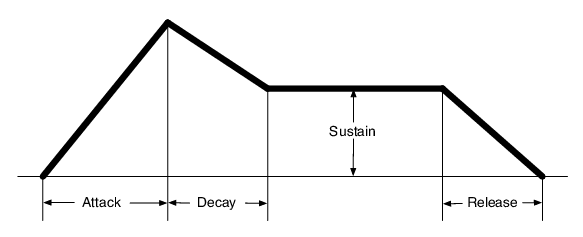
\includegraphics[scale=0.5]{graficos/adsr.png}
	\caption{Envolvente ADSR}
\end{figure}

Al sintetizar una nota utilizando esta envolvente y escuchar el sonido resultante, se nota un sonido pobre y lejano del que se podría escuchar en la realidad. Esto se debe a las discontinuidades abruptas que aparecen al aplicar cada uno de los segmentos correspondientes a cada parámetro.

Para hacer que sonido se asemeje más a uno real, se probó utilizar una envolvente del tipo ADSR pero con forma exponencial en lugar de que sea lineal.

Los resultados obtenidos fueron mas realistas que los resultados anteriores, el sonido no es mas suave, pero de todas formas le falta riqueza armónica.

\subsubsection{Envolvente en base a mustras}

Para obtener un sonido más realista, se obtuvieron las envolventes mediante muestras de una nota para cada instrumento, además de utilizar una envolvente distinta para cada armónico.


\subsection{Procedimiento}

Para sintetizar un instrumento, se tomó una muestra de una nota del instrumento elegido. A la muestra obtenida se le aplic\'o la transformada r\'apida de Fourier con el fin de poder analizar el contenido arm\'onico de la misma. De aqu\'i se sac\'o la informaci\'on de cu\'ales son los arm\'onicos que estan presentes en la señal, la amplitud y la fase de los mismos. La amplitud nos dice que tan fuerte va a sonar ese armónico y la fase es para conocer el desfasaje temporal que existe entre los diferentes componentes.

Para optimizar, se buscaron los picos con mayor amplitud, además de que éstos se encuentren separados con una distancia de aproximadamente la frecuencia fundamental, a tal forma de no tomar las componentes de ruido que aparecen en la muestra.

\begin{figure}[H]
	\centering
	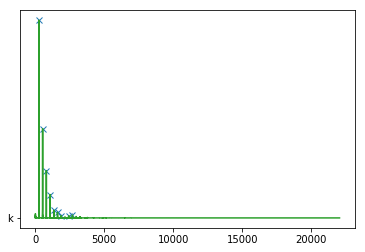
\includegraphics[scale=0.75]{graficos/fft.png}
	\caption{Transformada rápida de Fourier de la muestra con los picos utilizados para calcular la síntesis}
\end{figure}

Luego, para obtener la envolvente de cada armónico se utilizó la función 'spectrogram' de Python, de donde se obtiene la amplitud en función del tiempo para un cierto número de frecuencias, estas divididas en ``bines''. 
En base a esta información, teniendo en cuenta en que bin caía la frecuencia del armónico se calculó la envolvente de amplitud que correspondía, encontrando los picos máximos y realizando una interpolación de estos.

\begin{figure}[H]
	\centering
	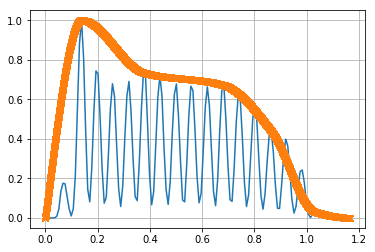
\includegraphics[scale=0.75]{graficos/envelope.png}
	\caption{Envolvente obtenida para un armónico}
\end{figure} 
\newpage
Finalmente se construye la nota a sintetizar mediante la ecuación \ref{eqn:additive}. A continuación se muestran la señal de entrada y la señal obtenida a la salida.

\begin{figure}[H]
\centering
  \begin{minipage}{0.4\textwidth}
    \centering
    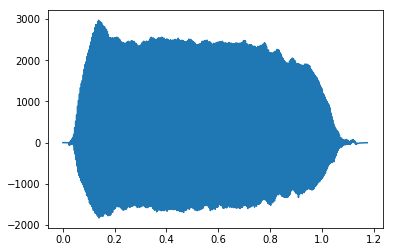
\includegraphics[width=1\textwidth]{graficos/entrada.png}
    \caption{Señal de entrada}
    \label{fig:uno}
  \end{minipage}%
  \hspace{5mm}
  \begin{minipage}{0.4\textwidth}
    \centering
    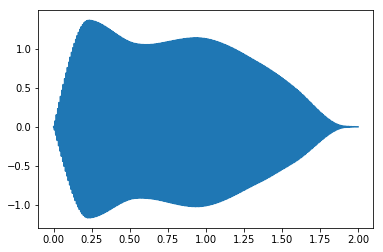
\includegraphics[width=1\textwidth]{graficos/salida.png}
    \caption{Señal de salida}
    \label{fig:dos}
  \end{minipage}
\end{figure}

La calidad del resultado obtenido depende de muchos parámetros. Las diferencias que se pueden observar entre la entrada y la salida se deben, por ejemplo, a que el número de armónicos tomados para el cálculo no coincide con el total, las envolventes calculadas para los parciales son una aproximacion a la envolvente real, lo cual generará mayor discrepancia entre el sonido usado de muestra y el sonido obtenido mediante la síntesis.

\subsection{Conclusiones}

Si bien el sonido obtenido es bueno ya que el método permite un gran control sobre todos los parciales, se encontraron limitaciones en este tipo de síntesis. Por ejemplo, la gran cantidad de parámetros que se necesitan para poder conseguir un sonido más real. Otra limitación que se puede notar al sintetizar notas de distintas duraciones, es que el sonido se empieza a distorsionar cuando la duración de la nota es muy corta, y es más notorio cuando la duración llega a ser menor que el tiempo de ataque.

También, otra limitación es el rango de frecuencias que puede generar un instrumento, lo que provocan que si se sintetizara una frecuencia que no se encuentre dentro de su rango no se escuchará un sonido representativo del instrumento. Además, al utilizar una única muestra por instrumento, al alejarse más de un cierto rango de la frecuencia de la misma, el sonido ya se empieza a distorsionar.

Luego, se pudieron notar ciertas similitudes en las envolventes de los distintos grupos de instrumentos, como por ejemplo los de cuerda, como el piano y la guitarra (no está incluída en el trabajo pero se estudió su muestra), donde el tiempo de ataque es muy corto y luego la amplitud decae sin tener casi un tiempo donde haya un nivel de sustain y otro ejemplo son los instrumentos de viento, donde el nivel de sustain se mantiene casi toda la duración de la nota.

\end{document}